\chapter{Implementación de la herramienta de Minería de Procesos \emph{Graph Miner}}\label{sec:chapterIV}
\addcontentsline{toc}{chapter}{Implementación de la herramienta de Minería de Procesos \emph{Graph Miner}}

\section{Uso de grafos como representación de los grupos}

Para dar una estructura de orden mínimo al comportamiento $B^g$, suponemos que es cierto lo siguiente: el resultado de la sesión $i$ depende en su mayor parte de lo ocurrido en la sesión $i-1$ o, como mucho, de cualquiera de las sesiones inmediatamente anteriores. Si aceptamos esta suposición, entonces $B^g$ tiene una estructura de orden parcial en la que cada sesión aparece conectada a la anterior.

Además, podríamos etiquetar estas relaciones con un número natural que indica el número de veces que esta relación se ha dado en $B^g$. De este modo se, obtiene el gráfico de la Figura \textbf{referencia}, un grafo totalmente conectado \textbf{revisar} que describe el camino seguido por los estudiantes con un sentido claro de las transiciones de un estado a otro. Esta Figura también cumple el factor de grado de entrada mencionado al principio: la suma de las aristas entrantes a un nodo coincide con el número de veces que el nodo aparece en el registro. No obstante, como este estudio se centra en el éxito y el fracaso de los alumnos, vamos a colapsar este grafo. Para simplificar las cosas sólo distinguiremos dos tipos de sesiones: las que fracasan, es decir, las que alcanzan los hitos $1$ a $4$, y las que tienen éxito, es decir, las que alcanzan el hito final $5$. Así pues, notaremos a las sesiones fallidas por $^sp_i^f$ y a las sesiones exitosas por $^sp_i^s$, como en la Figura \ref{fig:examples}, que continúa el ejemplo presentado en la Sección \ref{sec:initial}. Además, la matriz de adyacencia del segundo grafo puede verse en la Ecuación \ref{eq:adyacencia}.

\begin{figure}[H]
\centering
\subfloat[Grafo cíclico dirigido que captura las relaciones de precedencia entre las sesiones de la Tabla \ref{tab:sequence} ($16$ sesiones) obtenido colapsando los vértices de la misma en exitosas o fallidas. Los nodos con doble círculo representan sesiones en las que se ha resuelto un problema.]{\label{fig:examplecycles}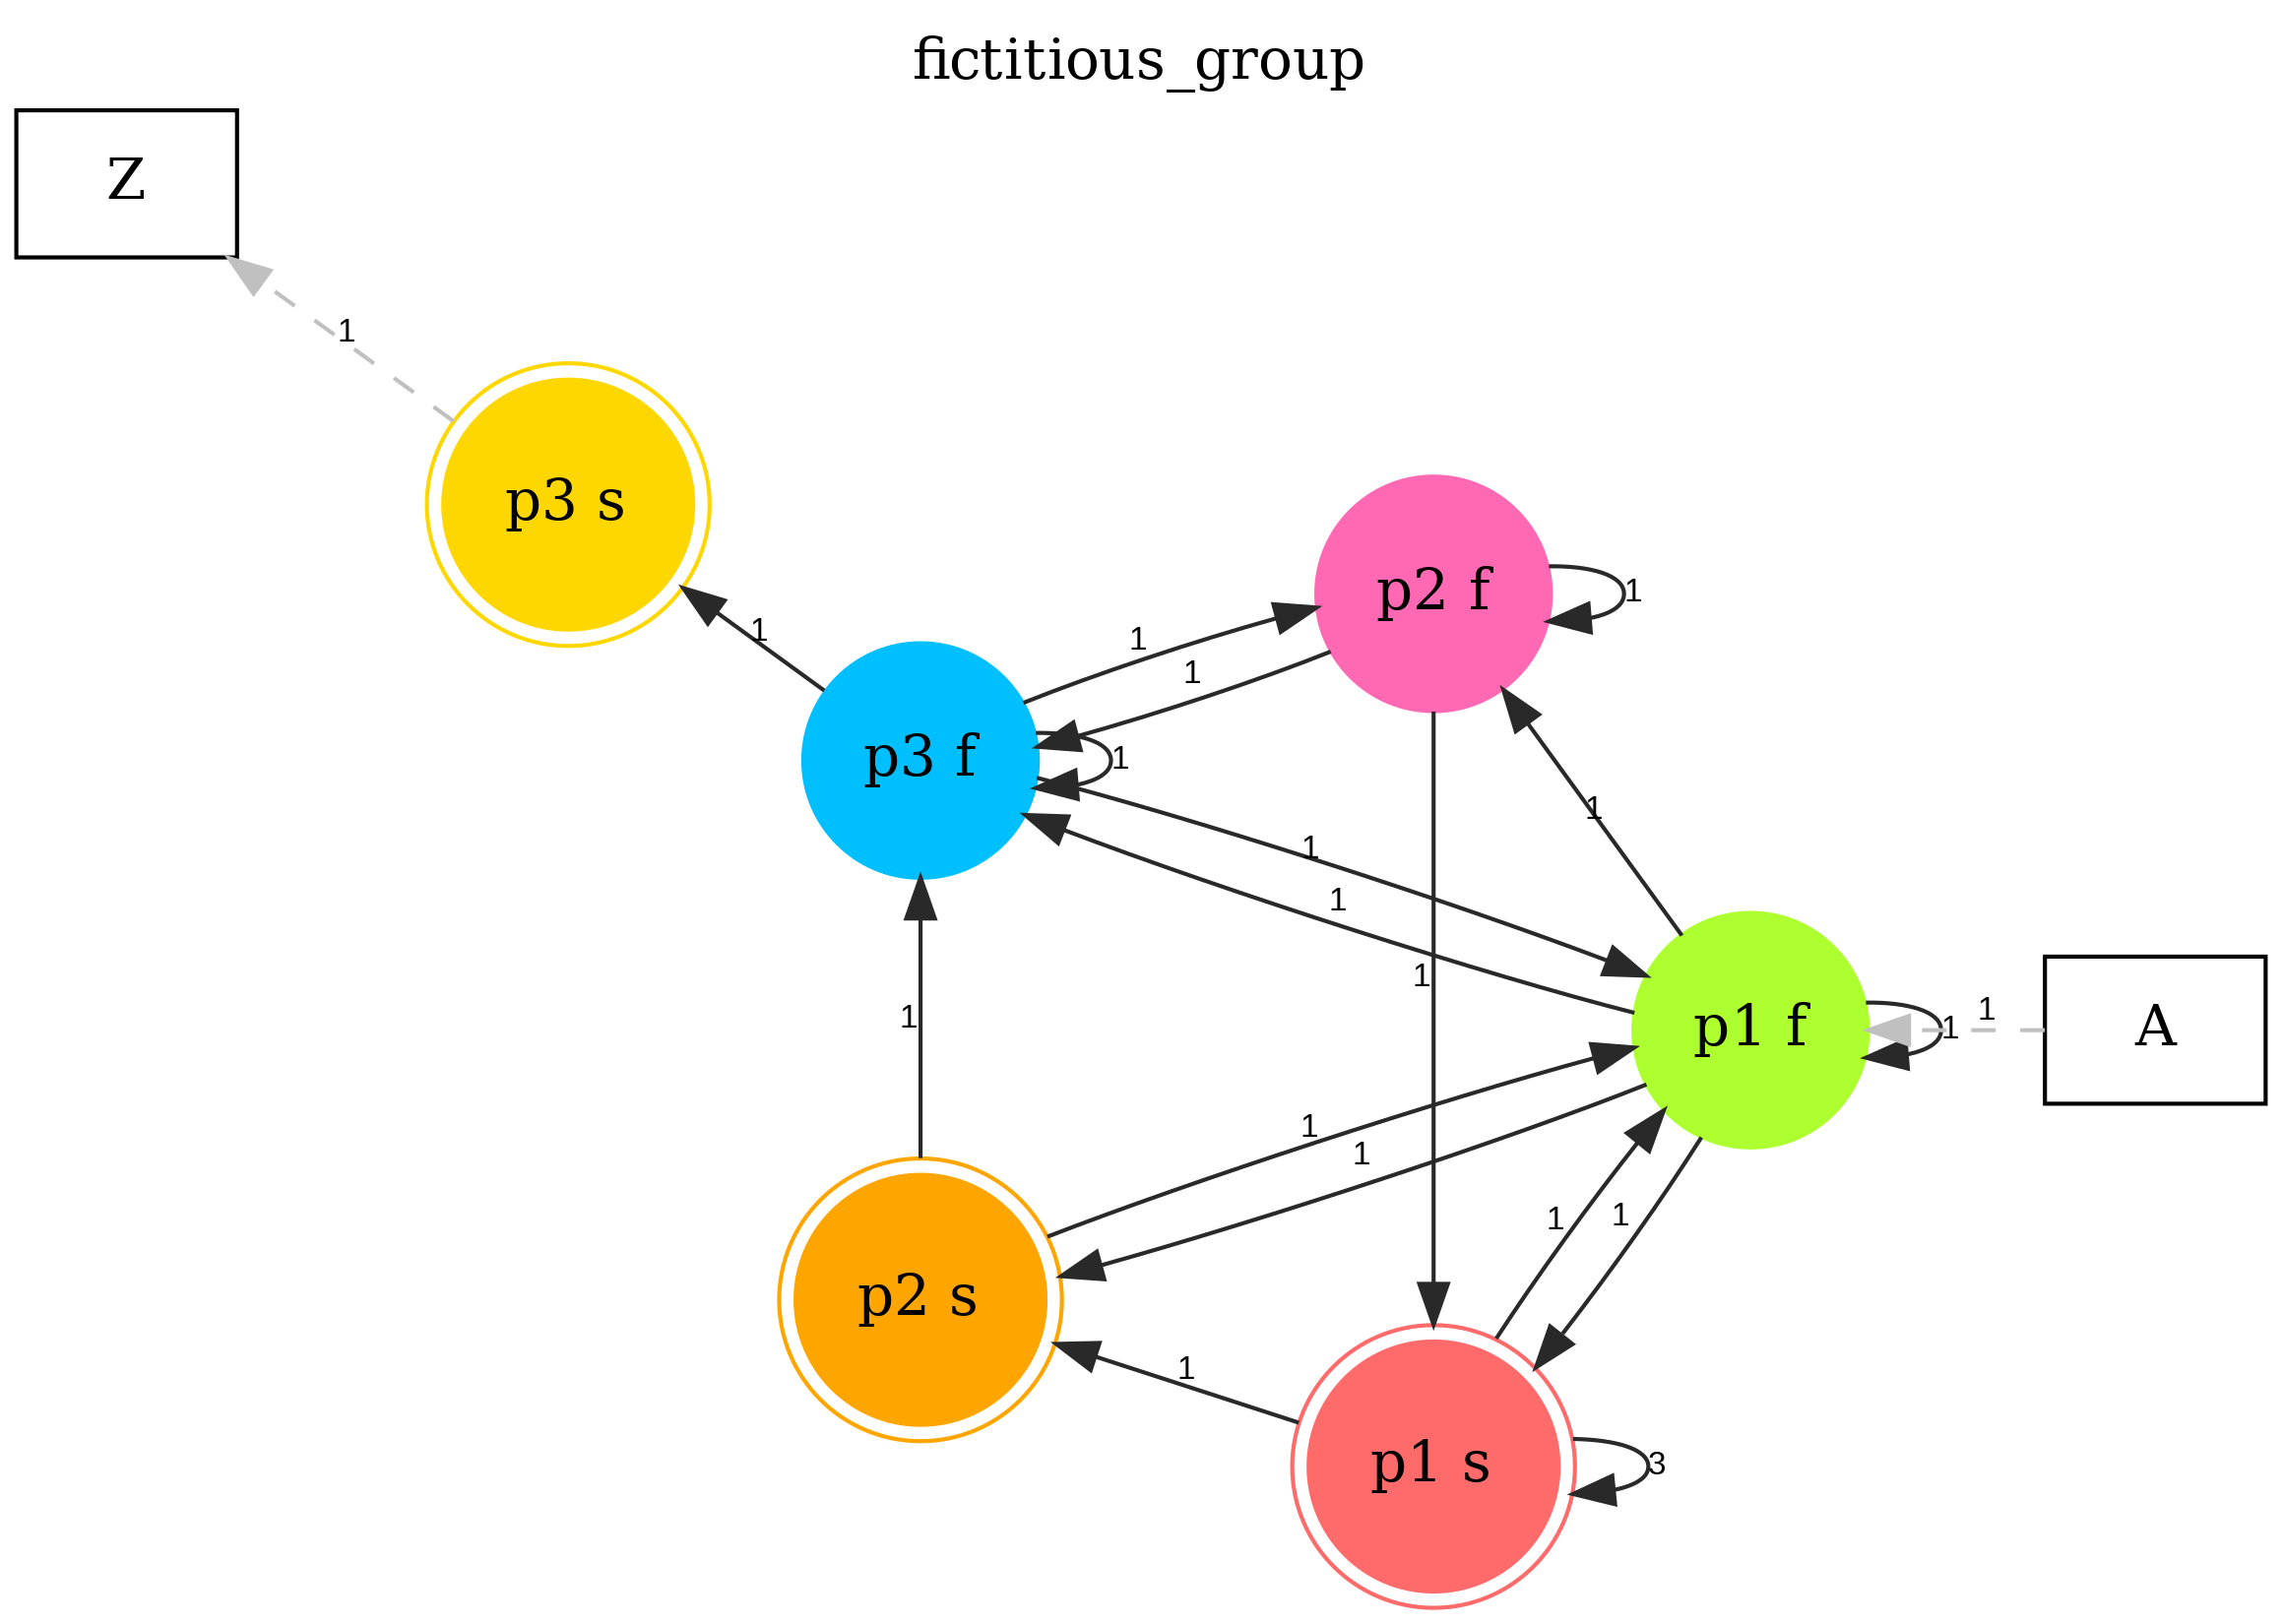
\includegraphics[width=0.47\textwidth]{implementación/examplecycles.png}}\qquad
\subfloat[El mismo grafo que el de la Figura \ref{fig:examplecycles} pero eliminando los ciclos
y manteniendo el mismo grado de entrada de cada vértice.]{\label{fig:examplewithoutcycles}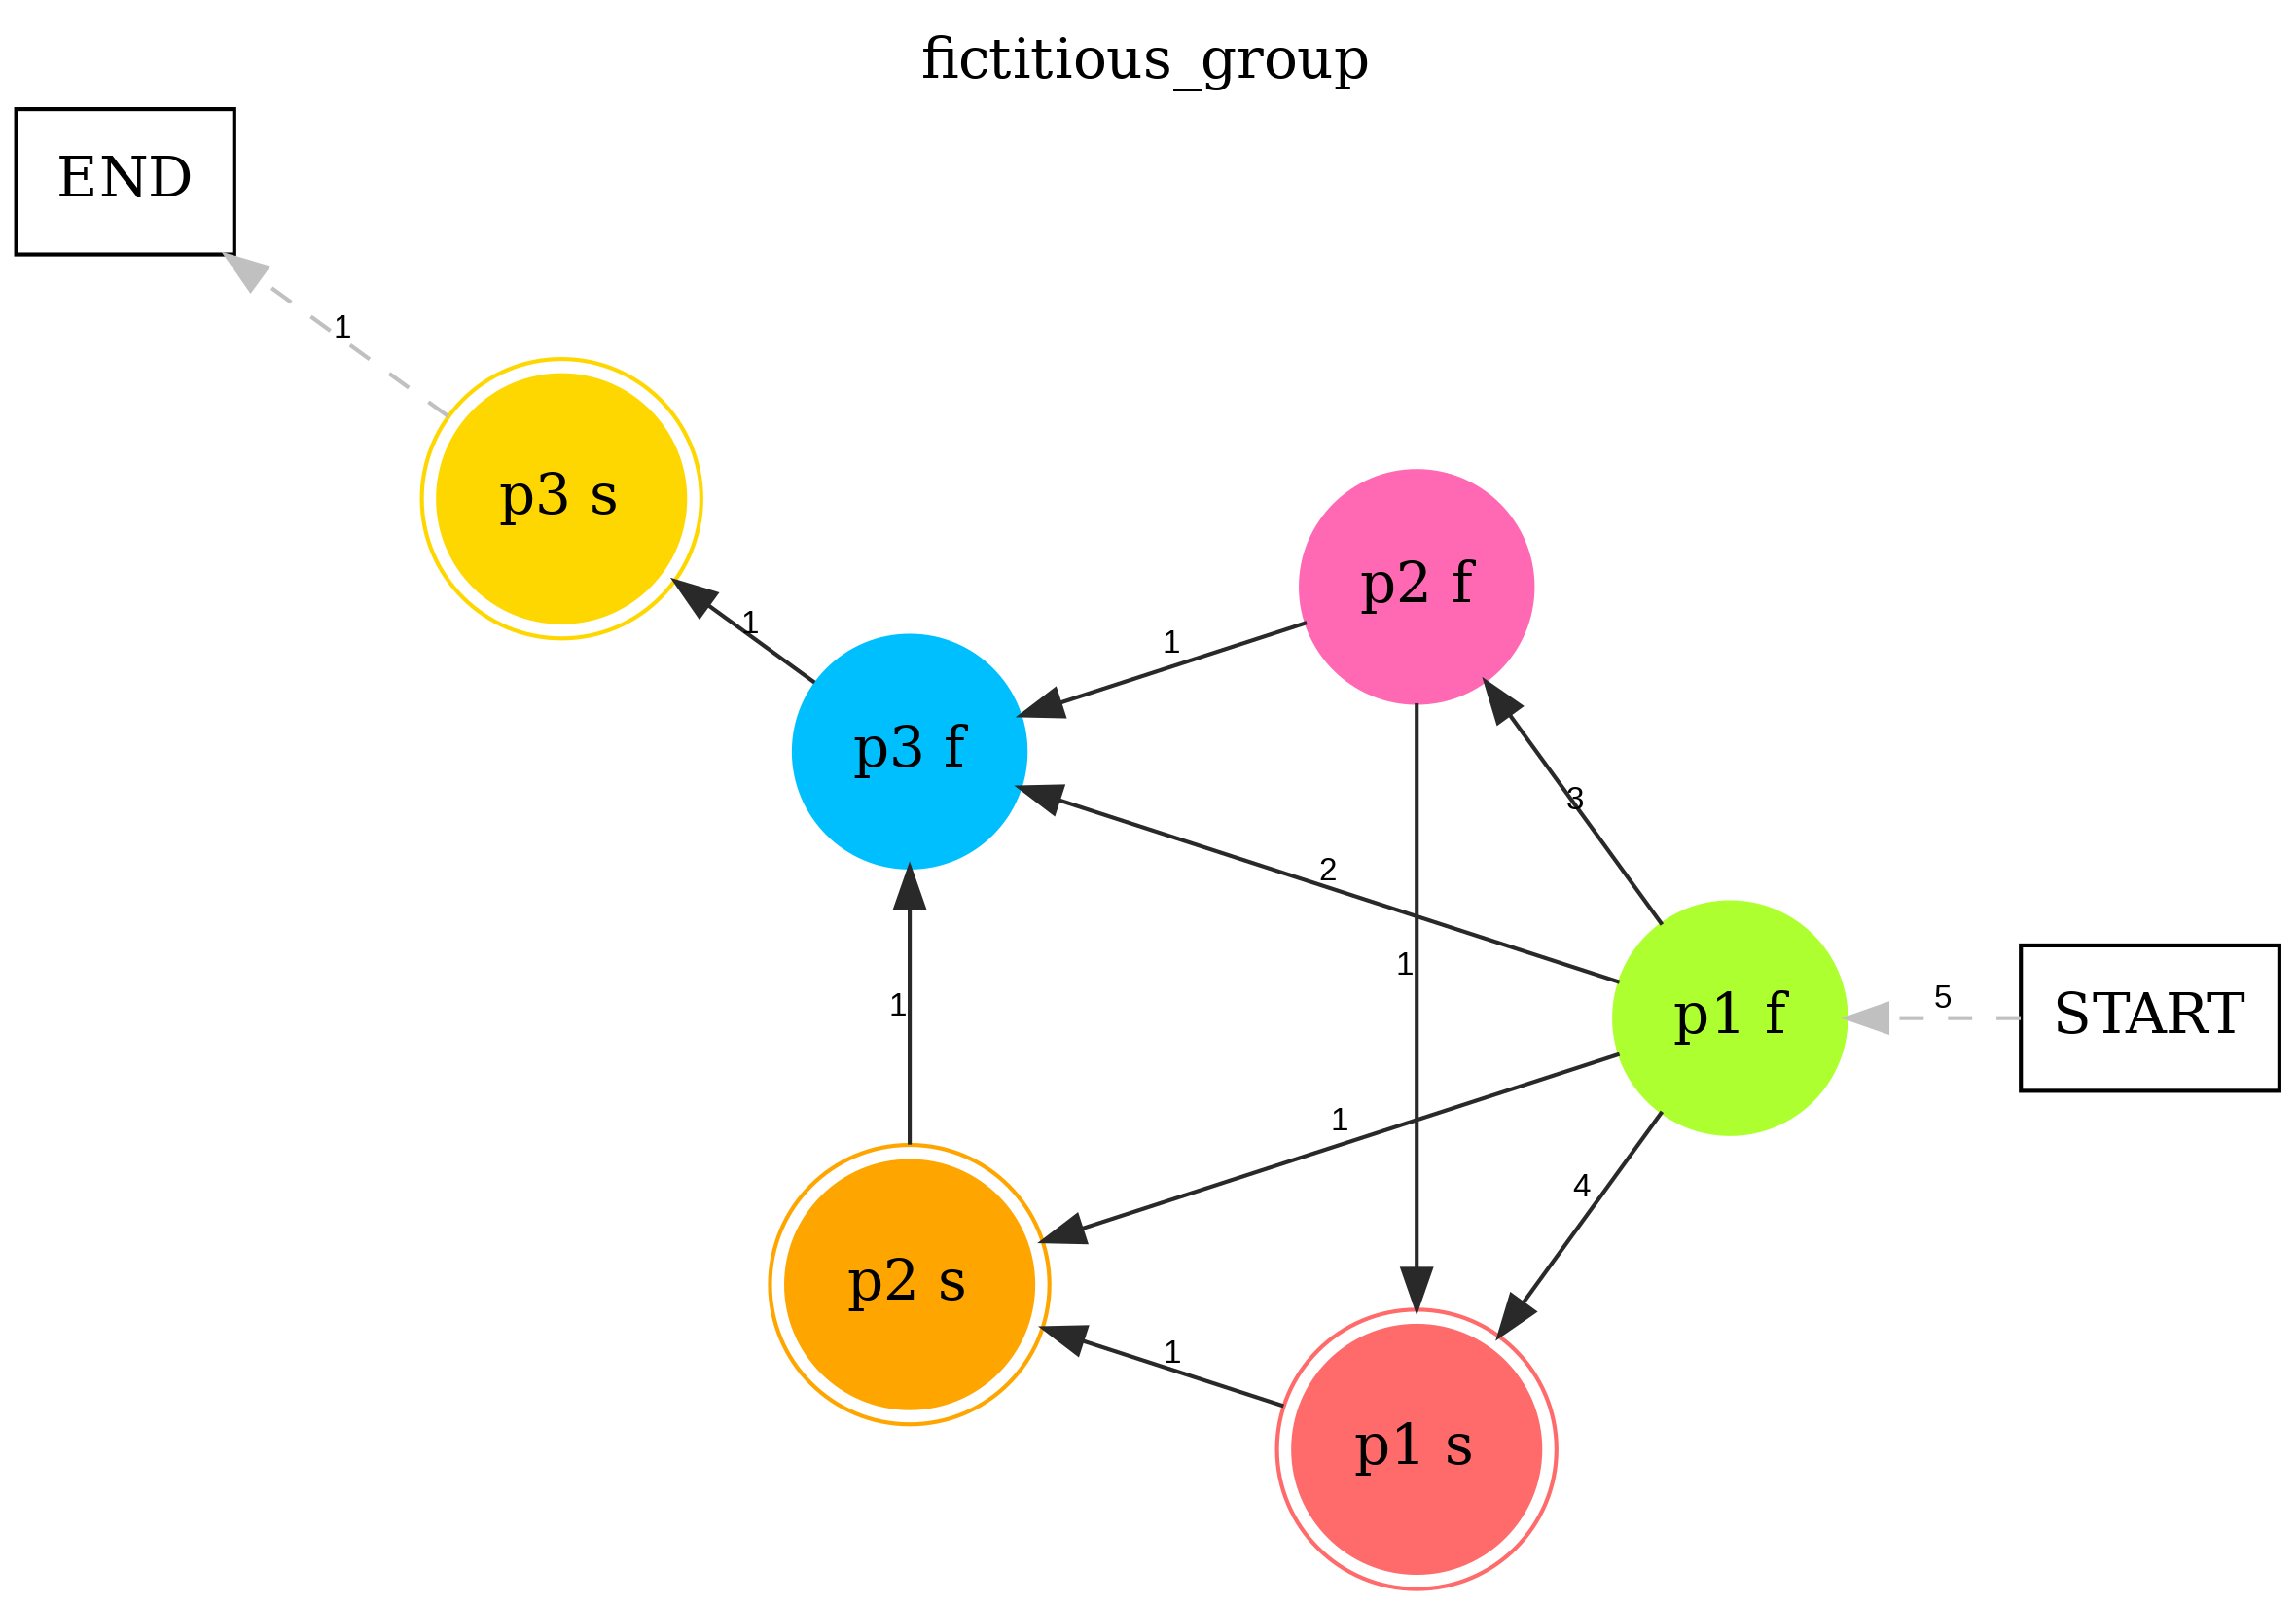
\includegraphics[width=0.47\textwidth]{implementación/examplewithoutcycles.png}}
\caption{Grafos resultantes de la continuación del ejemplo de la Sección \ref{sec:initial}.}
\label{fig:examples}
\end{figure}

\begin{equation}\label{eq:adyacencia}
\mathcal{A}^g = 
\left(
\begin{array}{c|cccccccc}
    & A & p_1^f & p_1^s & p_2^f & p_2^s & p_3^f & p_3^s & Z \\
  \hline
  A & \textbf{0} & 5 & 0 & 0 & 0 & 0 & 0 & 0 \\
  p_1^f & 0 & \textbf{0} & 4 & 3 & 1 & 2 & 0 & 0 \\
  p_1^s & 0 & 0 & \textbf{0} & 0 & 1 & 0 & 0 & 0 \\
  p_2^f & 0 & 0 & 1 & \textbf{0} & 0 & 1 & 0 & 0 \\
  p_2^s & 0 & 0 & 0 & 0 & \textbf{0} & 1 & 0 & 0 \\
  p_3^f & 0 & 0 & 0 & 0 & 0 & \textbf{0} & 1 & 0\\
  p_3^s & 0 & 0 & 0 & 0 & 0 & 0 & \textbf{0} & 1 \\
  Z & 0 & 0 & 0 & 0 & 0 & 0 & 0 & \textbf{0}
\end{array}
\right)
\end{equation}

Esta perspectiva nos permite ver $B^g$ como un grafo dirigido $G = (V^g,E^g)$ que capta la dinámica de un grupo mientras se esfuerzan por resolver los distintos problemas que se les han planteado. Por lo tanto, el conjunto de eventos (sesiones) que los estudiantes han realizado es el conjunto de vértices del grafo (\textbf{duda}):

\begin{equation}
V^g = \left\lbrace ^0A \right\rbrace \cup \left\lbrace ^sp_i^k \in B^g \right\rbrace
\end{equation}

y cada par de sesiones consecutivas se considera una arista del grafo:

\begin{equation}
E^g = \left\lbrace <x,y>, x = {}^sp_i^r, y = {}^tp_j^l, t = s+1, x,y \in B^g\right\rbrace
\end{equation}

que, de hecho, puede representarse como su matriz de adyacencia ponderada y que nos permite representar el invariante grado de entrada.

\section{La matriz característica de un grupo}

Este grafo sigue siendo un grafo cíclico (Definición \ref{def:cyclic}) y, como estamos interesados en la representación más esencial del comportamiento de los estudiantes, también eliminamos esos ciclos quitando una cantidad mínima de aristas y conservando la invariante del grado de entrada, obteniendo el grafo esencial de la Figura \ref{fig:examplewithoutcycles}, con su respectiva matriz de distancias (Ecuación \ref{eq:adyacencia}), que denominamos matriz característica (Definición \ref{def:adjacency}) del grupo $g$, $\mathcal{A}^g$. Esta matriz característica es una representación minimal de $B^g$ y a partir de ella se pueden extraer numerosas métricas, siendo la más importante una medida de la complejidad inherente a $B^g$.

Por lo tanto, $\mathcal{A}^g[x,y] = d > 0$ significaría que $x$ precede a $y$ $d$ veces en $B^g$. Así pues, cuanto mayor sea $d$, mayor será la influencia de $x$ sobre $y$ en términos del comportamiento codificado en $\mathcal{A}^g$. En aras de la simplicidad, además del uso de valores enteros para obtener una fila o columna, también podrían utilizarse sus nombres como, por ejemplo, se muestra en la Ecuación \ref{eq:example}.

\begin{equation}\label{eq:example}
\mathcal{A}[1,2] = \mathcal{A}[p_2^f,p_3^f] = 4
\end{equation}

Podría decirse que $\mathcal{A}^g$ contiene lo que podría haber sido la \emph{experiencia} de resolver todos los problemas, es decir, una especie de huella que codifica la relación entre fracaso y éxito y la fuerza de estas relaciones. Vale la pena decir que en todo el registro de la Tabla I todas estas matrices son diferentes entre sí. Se derivarán otras dos matrices de $\mathcal{A}^g$. En primer lugar, obtendremos la matriz de adyacencia característica $\mathcal{A}'[r, c]$ que es $1$ sólo cuando $\mathcal{A}[r, c] > 0$. En segundo lugar, calcularemos la matriz de distancia mínima que se ha obtenido aplicando el camino más corto de Dijkstra, de modo que $\hat{\mathcal{A}}[r, c]$ contiene una especie de longitud de camino mínima entre ambos nodos del grafo en función del número de sesiones. Por tanto, estas estructuras son un punto de partida ideal desde el que decodificar la información sobre esta experiencia, en particular para validar si esta estructura puede estar relacionada con el éxito o no de cada grupo. Es decir, ¿un mal comportamiento de los alumnos produciría un grafo mal estructurado? Y viceversa, ¿las medidas estándar de calidad y entropía definidas puramente sobre grafos permiten detectar grupos en riesgo?
Y, la respuesta, resulta ser sí (Sección ).

\section{Resultados obtenidos}

Comparando las Figuras \ref{fig:DBA1516P2GA1} y \ref{fig:problemsDBA1516P2GA} vemos que el diagrama de la implementación propia y el original obtenido con Disco coinciden.

\begin{figure}[H]
    \centering
    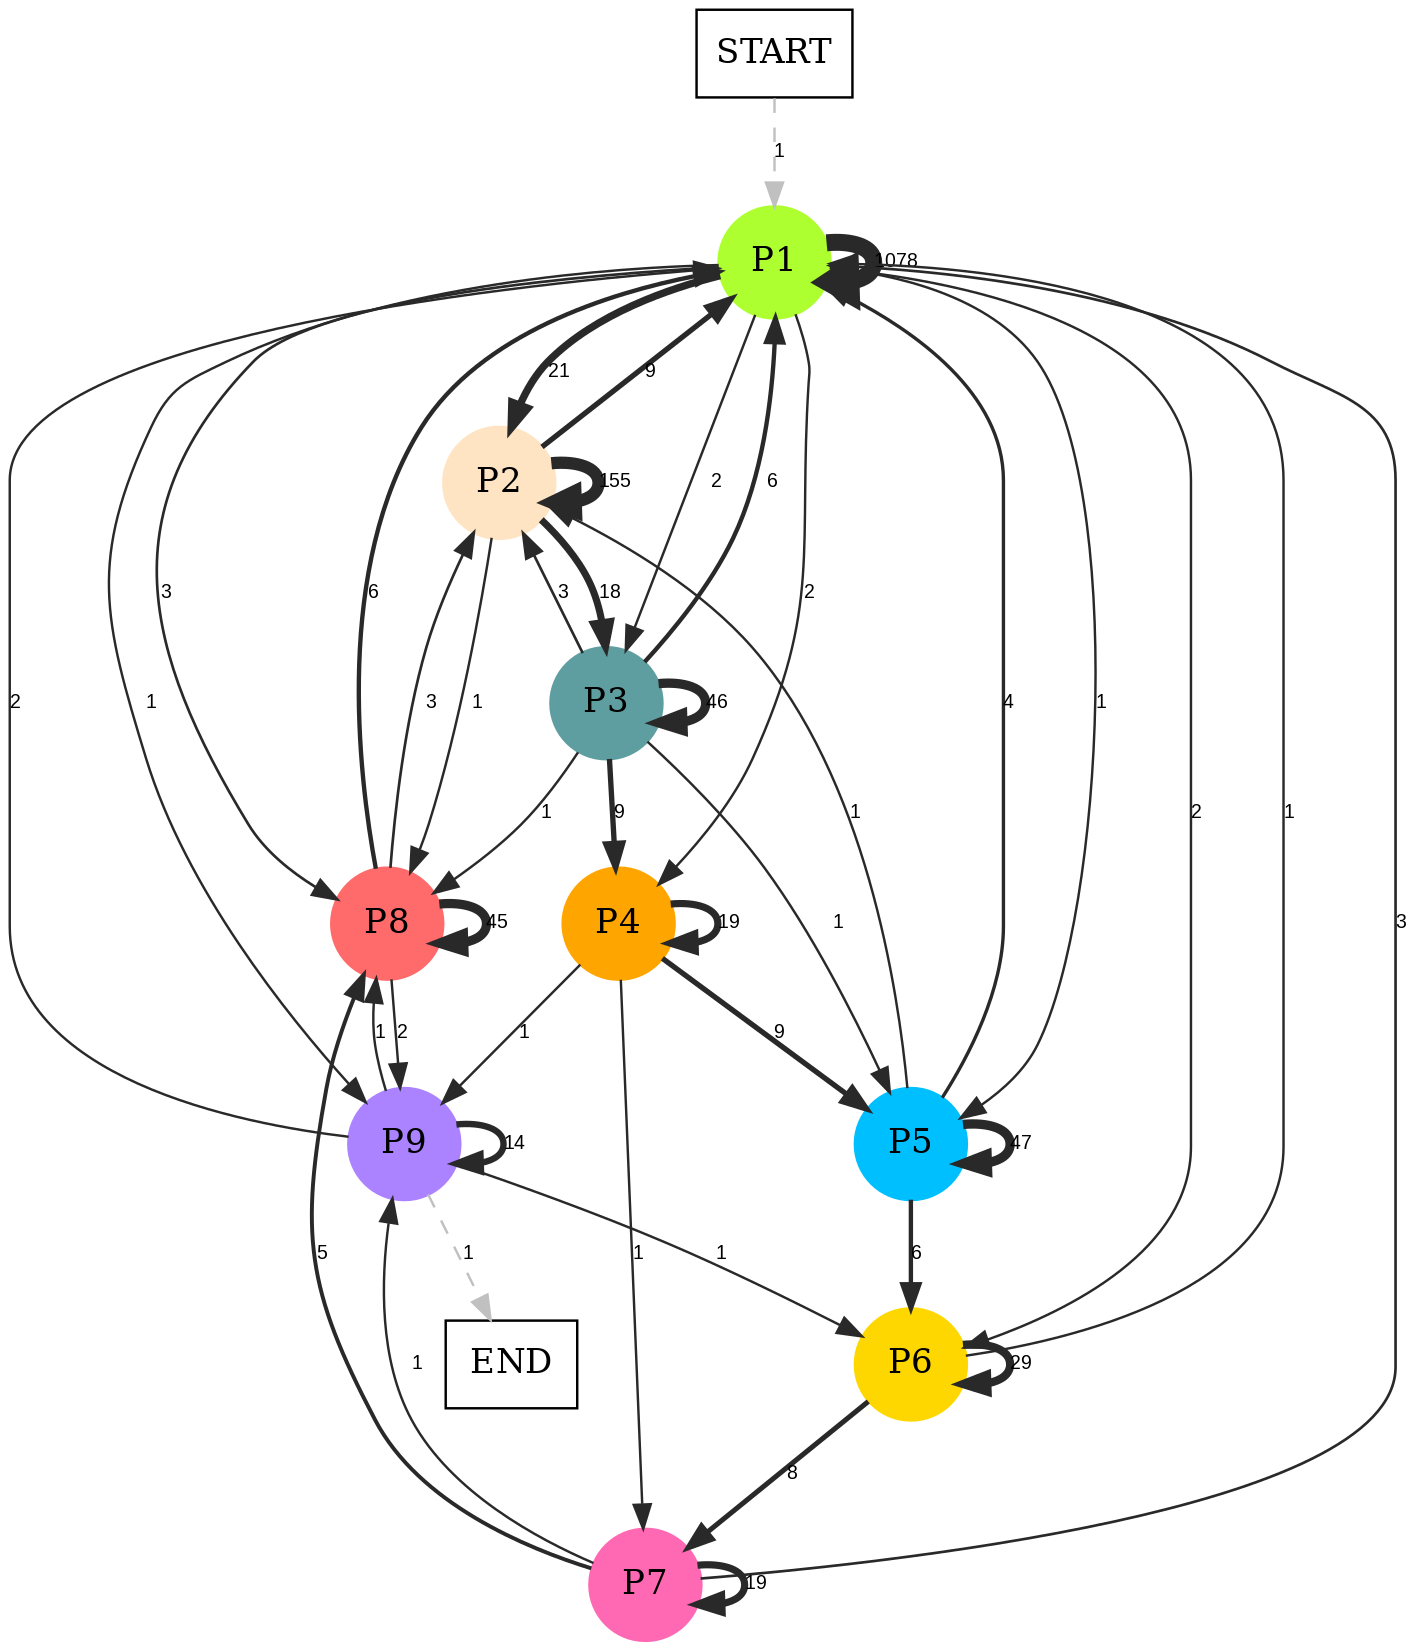
\includegraphics[width=0.5\textwidth]{DBA1516P2GA1.png}
    \caption{Análisis de procesos del grupo \texttt{DBA 1516 P2 GA} (\texttt{Activity} problema y \texttt{CaseId} grupo) obtenido con la implementación propia.}
    \label{fig:DBA1516P2GA1}
\end{figure}

Además, como podemos ver en la Figura \ref{fig:DBA1516P2GA2}, hemos obtenido el mismo diagrama que en el de la Figura \ref{fig:compoundDBA1516P2GA} con la salvedad de que hemos impedido el retorno a un estado anterior (el motivo se verá más adelante). Es decir, se han eliminado ciclos.

\begin{figure}[H]
    \centering
    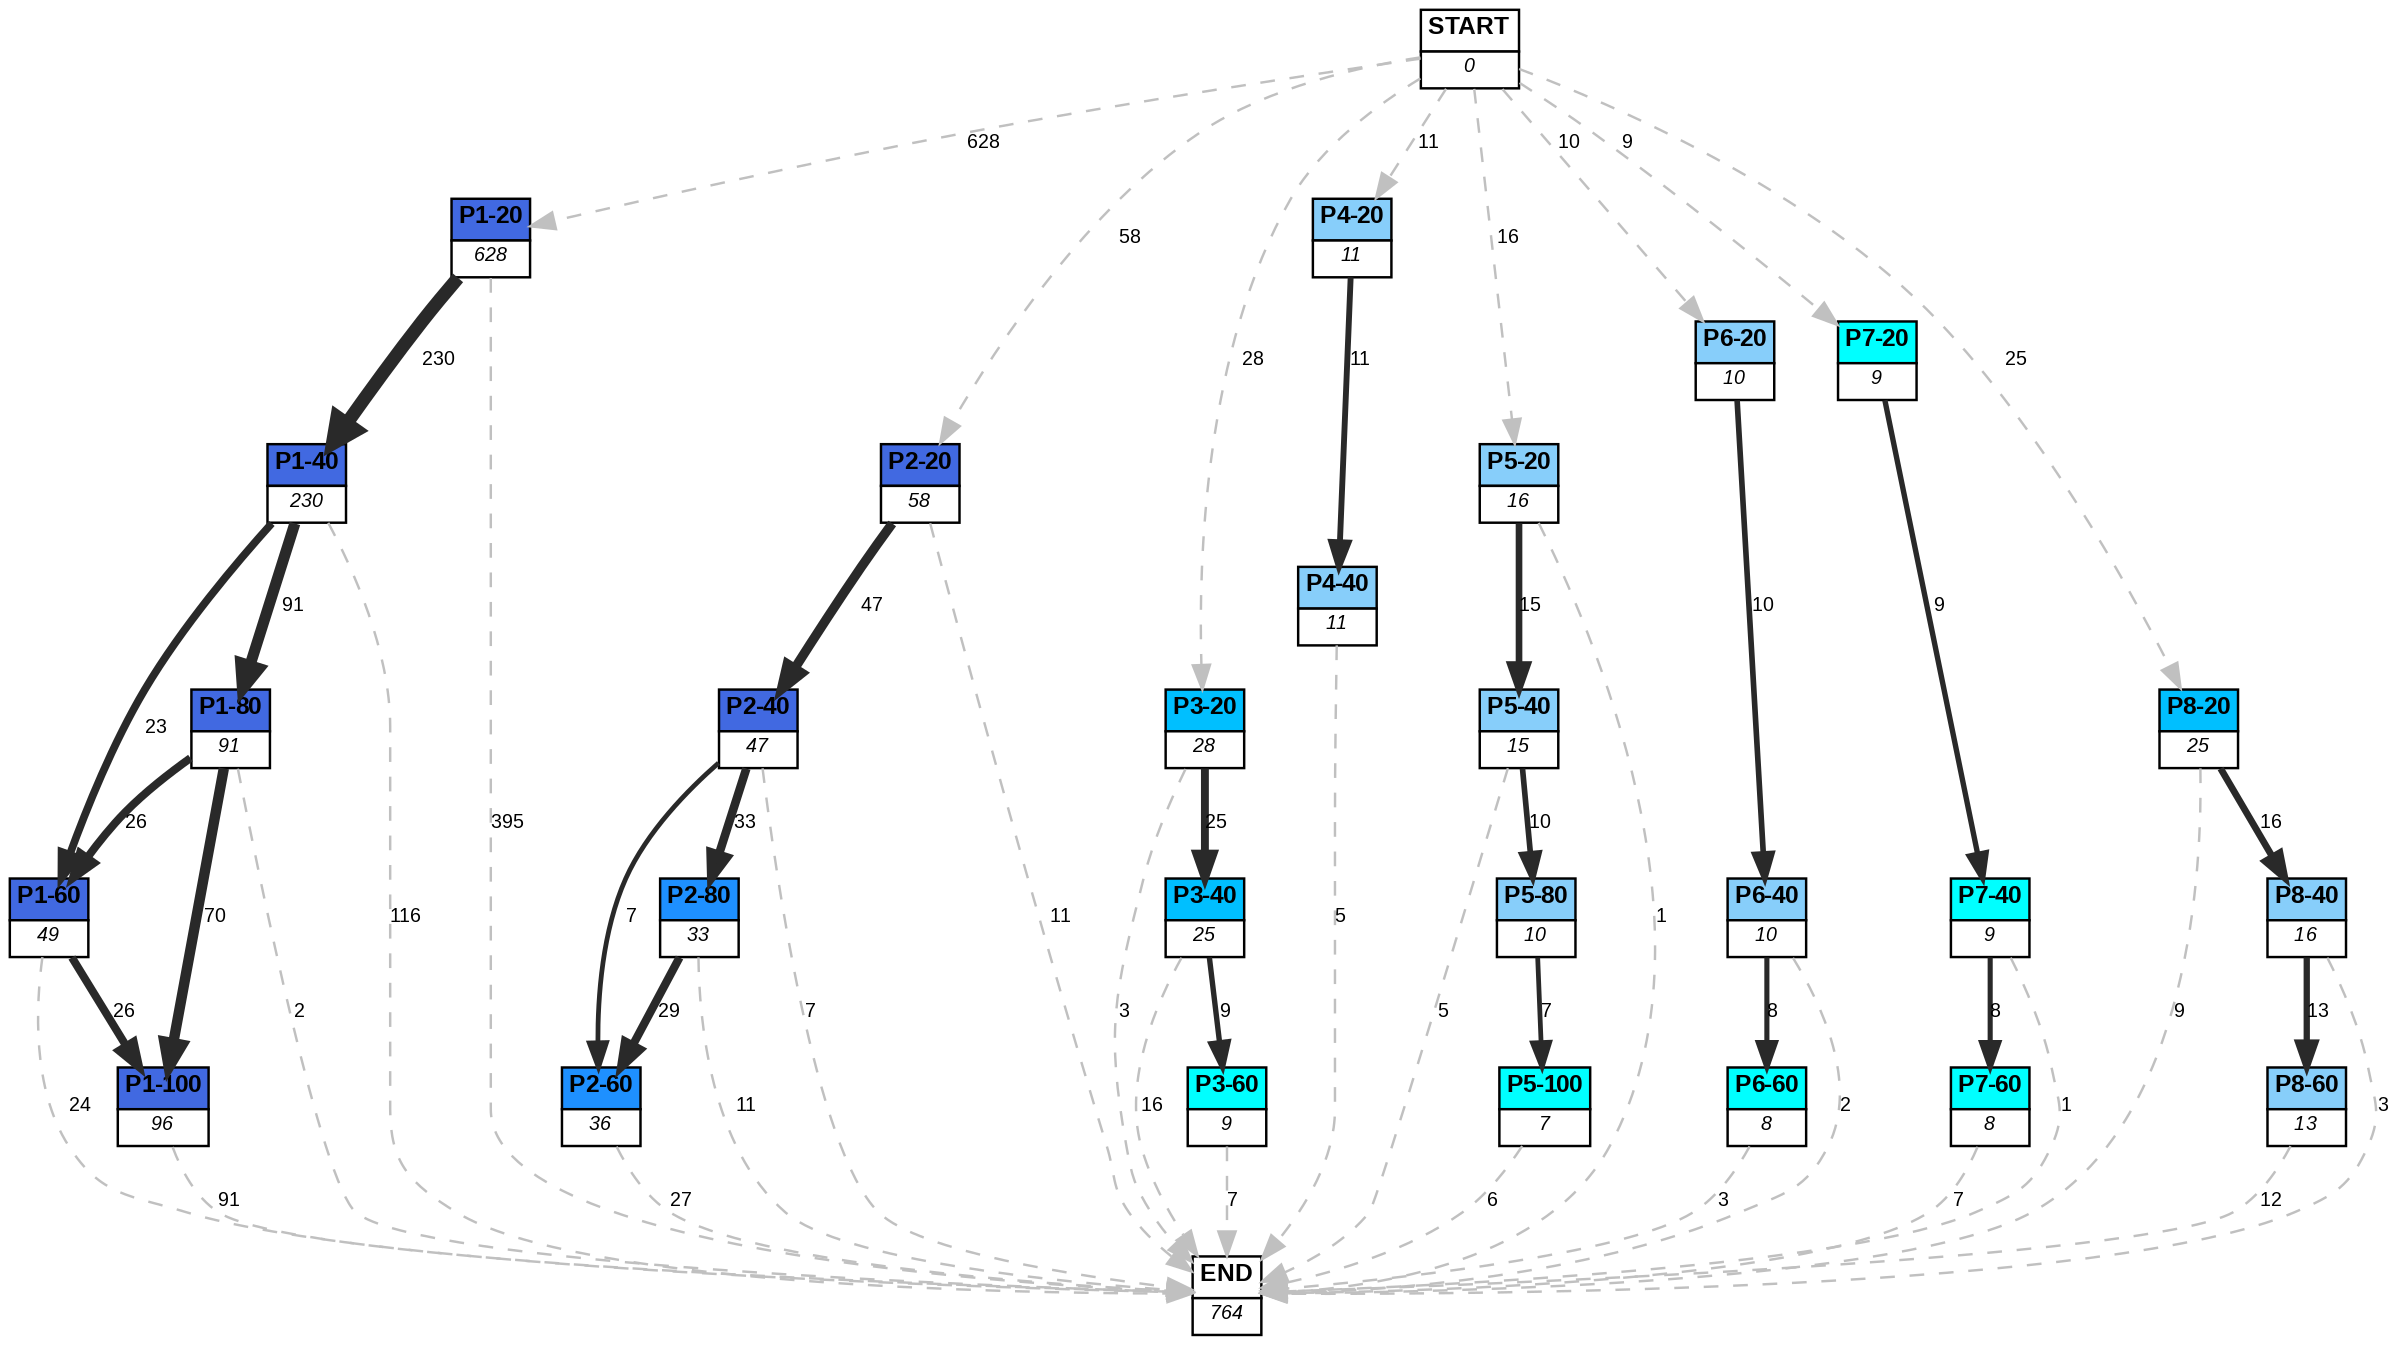
\includegraphics[width=\textwidth]{DBA1516P2GA2.png}
    \caption{Análisis de procesos del grupo \texttt{DBA 1516 P2 GA} (\texttt{Activity} problema-milestone y \texttt{CaseId} sesión) obtenido con la implementación propia.}
    \label{fig:DBA1516P2GA2}
\end{figure}

Además, se ha extendido la implementación de la herramienta de minería de procesos Disco \cite{gunther2012disco}, obteniendo otros diagramas que nos serán de mucha utilidad, como la agrupación en estados exitosos y fallidos (Figura) y una serie de grafos parciales considerando sólo la resolución hasta el problema $i$-ésimo, $i \in \left\lbrace 1,\dots,9 \right\rbrace$ (Figura).

A partir de ahora, estos diagramos tendrán la consideración de grafos. En particular, serán grafos dirigidos y operaremos con ellos como tales. En el siguiente capítulo se expondrán los conceptos básicos de grafos y principales resultados matemáticos que se usarán en este trabajo fin de grado.